\section{RMSE vs Spike Rate for Constant Driving Force}
\label{section:analysis:sc_rmse}



We analyse the network described by equations (\ref{eq:rotated_voltage_dynamics}) and (\ref{eq:rho_dot}) for the case of a constant (in time) driving force $\tilde{c}(\xi) = \tilde{c}$. \\

\subsection{Ideal Network}
We assume the network 



\subsection{Neuron Trajectories}
Consider the dynamical system 
$$
\dot{y} = \Lambda y + \beta \tilde{c}, \hspace{4mm} y(0) = y_0
$$
as implemented by the network of $N$ neurons whose encoding directions are
$$
\begin{bmatrix}
S & 0
\end{bmatrix} \in \mathbf{R}^{d \times N},
$$
where

$$S = \begin{bmatrix}
S_1 & \hdots & S_d
\end{bmatrix} \in \mathbf{R}^{d \times d}$$
is a diagonal matrix.\\


Let $$\tilde{c} =  k \hat{u} \in \mathbf{R}^d$$ such that
\begin{align*}
-\Lambda^{-1} \beta (k \hat{u}) &= k \frac{S_j}{||S_j||}
\\
\\
\implies
\tilde{c} &= -\frac{k}{||S_j||} \beta^{-1} \Lambda S_j.
\end{align*}

With this choice of $\tilde{c}$,  if we assume neuron $j$ spikes periodically at a rate $\phi_j$. 

\subsection{Solution for the Periodically Spiking Network}

 Assume the spike train $\tilde{o}_j$ is a periodic sequence of impulses spaced in time by $\frac{1}{\phi_j}$. If the first spike occurs at $\xi_j^0 = 0$, then $\tilde{o}_j(\xi) = \sum_{l=0}^{\infty} \delta \left(\xi-\frac{l}{\phi_j}\right).$ By our choice of $k$, only neuron $j$ will spike so that 

\begin{align}
\label{eq:estimation_dynamics_const_driving}
\dot{\hat{y}}(\xi) = - \hat{y} + \sum_{l=0}^{\infty} \delta \left(\xi_j^k - \frac{l}{\phi_j}\right) \, S_j .
\end{align}

Equation (\ref{eq:estimation_dynamics_const_driving}) implies that the network estimate $\hat{y}$ will decay until $j$'s first spike  occurs at $\xi_j^1 = \frac{1}{\phi_j}$. 
\begin{align*}
\hat{y}(\xi) = \hat{y}(0) e^{-\xi}, \hspace{4mm} 0 \leq \xi < \frac{1}{\phi_j}.
\end{align*}


 At this instant, $S_j$ is added to neuron $j$'s component of the estimate.
 \begin{align*}
 \hat{y}( \frac{1}{\phi}) =  \hat{y}(0) e^{- \frac{1}{\phi}} + S_j.
 \end{align*}
 
Decay again occurs until the next spike
\begin{align*}
\hat{y}(\xi) &= \hat{y}(\frac{1}{\phi_j}) e^{-(\xi - \frac{1}{\phi_j})}, \\
\\
&= 
\left( \hat{y}(0) e^{- \frac{1}{\phi_j}} + S_j \right)e^{-(\xi - \frac{1}{\phi_j})} , \hspace{4mm} 
\frac{1}{\phi_j} \leq \xi < \frac{2}{\phi_j}\\
\\
\implies
\hat{y}(\frac{2}{\phi_j}) &= \left(\hat{y}(0)e^{- \frac{1}{\phi_j}} + S_j \right) e^{-\frac{1}{\phi_j}} + S_j\\
\\
&= x(0)
e^{-\frac{2}{\phi}} + S_j e^{-\frac{1}{\phi_j}} 
+ S_j.
\end{align*}

The third spike more clearly shows the recursive behavior
\begin{align*}
\hat{y}(\frac{3}{\phi_j}) &= \left[\hat{y}(0)
e^{-\frac{2}{\phi_j}} + S_j e^{-\frac{1}{\phi_j}} 
+ S_j\right] e^{-\frac{1}{\phi_j}} + S_j\\
\\
&= \hat{y}(0) e^{-\frac{3}{\phi_j}} + S_j e^{-\frac{2}{\phi_j}} 
+ S_j e^{-\frac{1}{\phi_j}} + S_j
\end{align*}
Let us consider the $n^{th}$ spike sufficiently far from $\xi=0$ such that the transient term $\hat{y}(0)e^{-\frac{n}{\phi_j}}$ can be neglected. This leads to the expression

\begin{align*}
\hat{y}(\frac{n}{\phi_j}) &= \sum_{l=0}^{n-1} S_j e^{- \frac{l}{\phi_j}}  \\
\\
&= S_j \frac
{ 1 - e^{-\frac{n}{\phi_j}}  }
{ 1 - e^{-\frac{1}{\phi_j}}  }.
\end{align*}

For sufficiently large $n$, this converges to 
$$
\hat{y}(\xi_1^n) = \frac{S_j}{1 - e^{-\frac{1}{\phi_j}}}.
$$



We know from equation (\ref{eq:estimation_dynamics_const_driving}) that the estimate will decay exponentially from this value over an interval $\frac{1}{\phi_j}$ until a spike returns it returns to the initial value. Thus we have an explicit expression for the long-term behavior given by 

\begin{equation}
\label{eq:const_driving_network_estimate_explicit_expression_long_term_phi}
\hat{y}(\xi) =
\frac{S_j}{1 - e^{-\frac{1}{\phi_j}}} e^{- (\xi) \mod{\frac{1}{\phi_j}}},
\end{equation} 
where $x \mod{y}$ denotes the fractional remainder of $x$ after division by $y$. 







\subsection{ RMSE for Periodic Spiking} From equation (\ref{eq:const_driving_network_estimate_explicit_expression_long_term_phi}) the error $\epsilon = y - \hat{y}$ is a periodic function of $\xi$ with period $\frac{1}{\phi_j}$. 

Assume 
\begin{align*}
 \dot{y} &= 0 
 \\
 \\
 \implies y(\xi) &= k \frac{S_j}{||S_j||}.
\end{align*}
 
We compute the  RMSE of the error signal  $\epsilon$ by 
\begin{equation}
\label{eq:per_spike_rmse_def}
RMSE = \sqrt{\phi_j \int_{0}^{\frac{1}{\phi_j}} \!  ||\epsilon(\tau)||^2 \, \, \mathrm{d}\tau}.
\end{equation}

The integrand simplifies to 

\begin{align*}
||\epsilon||^2  &= (y_j - \hat{y})^2 
\\
\\
&= ||y||^2 - 2 y^T\hat{y} + ||\hat{y}||^2
\\
\\
&= k^2 - 2  \frac{k \, ||S_j||}{1 - e^{-\frac{1}{\phi_j}}} e^{-\tau}  + \frac{||S_j||^2}{\left(1 - e^{-\frac{1}{\phi_j}}\right)^2}e^{-2\tau}
\\
\\
\end{align*}

Note that
$$
\int_{0}^{\frac{1}{\phi_j}} \! e^{-\tau} \, \, \mathrm{d}\tau 
=
1-e^{-\frac{1}{\phi_j}},
$$

while 
\begin{align*}
\int_{0}^{\frac{1}{\phi_j}} \! \left(e^{-\tau}\right)^2
&=
\frac
{
	1 - e^{-\frac{2}{\phi_j}}
}
{2}
\\
\\
&= 
\frac{1}{2}\left(1 - e^{-\frac{1}{\phi_j}}\right) \left(1 + e^{-\frac{1}{\phi_j}}\right).
\end{align*}

Therefore the integral is

\begin{align*}
\phi\int_{0}^{\frac{1}{\phi}} \!  \epsilon_j(\tau)^2 \, \, \mathrm{d}\tau 
&= 
k^2  - 
 2  \phi \, k \, ||S_j|| +
  \phi_j \frac{||S_j||^2}{2} \frac{1 + e^{-\frac{1}{\phi_j}}}{1 - e^{-\frac{1}{\phi_j}}}.
\end{align*}


The  RMSE of the network estimate is thus
\begin{equation}
\label{eq:constant_driving:per_spike_rmse_full}
RMSE =
\sqrt
{
k^2 - 
 2  \phi \, k \, ||S_j|| +
  \phi_j \frac{||S_j||^2}{2} \frac{1 + e^{-\frac{1}{\phi_j}}}{1 - e^{-\frac{1}{\phi_j}}}
}.
\end{equation}

Note $\phi_j$ is dependent on the remaining parameters. We wish to reduce equation (\ref{eq:constant_driving:per_spike_rmse_full}) to a function of independent variables. The rate $\phi_j$ had no analytic solution from the voltage trajectory, but can be deduced from equation (\ref{eq:const_driving_network_estimate_explicit_expression_long_term_phi}). Consider the network estimate immediately before a spike occurs, i.e

$$
\hat{y}(\xi^{-}) = \frac{S_j}{1 - e^{-\frac{1}{\phi}}} e^{-\frac{1}{\phi}}.
$$

At this point, the error induces a spike in neuron $j$, i.e.

$$
 v(\xi) = S_j \epsilon = v_{th} = \frac{||S_j||^2}{2}.
$$

This implies 

\begin{align*}
\frac{||S_j||^2}{2} 
&=
S_j^T\left( y-\hat{y}\right)
\\
\\
&=
||S_j||^2\left( \frac{k}{||S_j||}  - \frac{e^{-\frac{1}{\phi_j}}}{1 - e^{-\frac{1}{\phi_j}}}\right).
\\
\\
&=
||S_j||^2\left( \frac{k}{||S_j||}   - \frac{1}{e^{\frac{1}{\phi_j}} - 1}\right).
\\
\\
\implies
e^{\frac{1}{\phi}} - 1
&=
\frac{1}{
\frac{k}{||S_j||}  - \frac{1}{2}}
\\
\\
\implies
\frac{1 + e^{-\frac{1}{\phi}}}{1-e^{-\frac{1}{\phi}}} 
&=
\frac{2\,k}{||S_j||}.
\end{align*}

Substitute this last expression into equation (\ref{eq:constant_driving:per_spike_rmse_full}) to get

\begin{align*}
RMSE_{j} 
&=
\sqrt
{
k^2 - 
4 \, \phi \, k^2 \frac{1 - e^{-\frac{1}{\phi_j}}}{1 + e^{-\frac{1}{\phi_j}}} + 2 \, \phi_j \, k^2 \, \frac{1 - e^{-\frac{1}{\phi_j}}}{1 + e^{-\frac{1}{\phi_j}}}
}
\\
\\
&=
k \sqrt
{
1 - 2 \, \phi_j \,  tanh\left(\frac{1}{2\phi_j}\right)
}.
\end{align*}

Finally, we can normalize by $k$ to obtain the  NRMSE that is both dimensionless and solely dependent on the firing rate. 

\begin{align}
\label{eq:const_driving:per_spike_rmse_phi}
NRMSE_{j}(\phi_j) = \sqrt
{
1 - 2 \, \phi_j \,  tanh\left(\frac{1}{2\phi_j}\right)
}. 
\end{align}


\begin{figure}
\centering
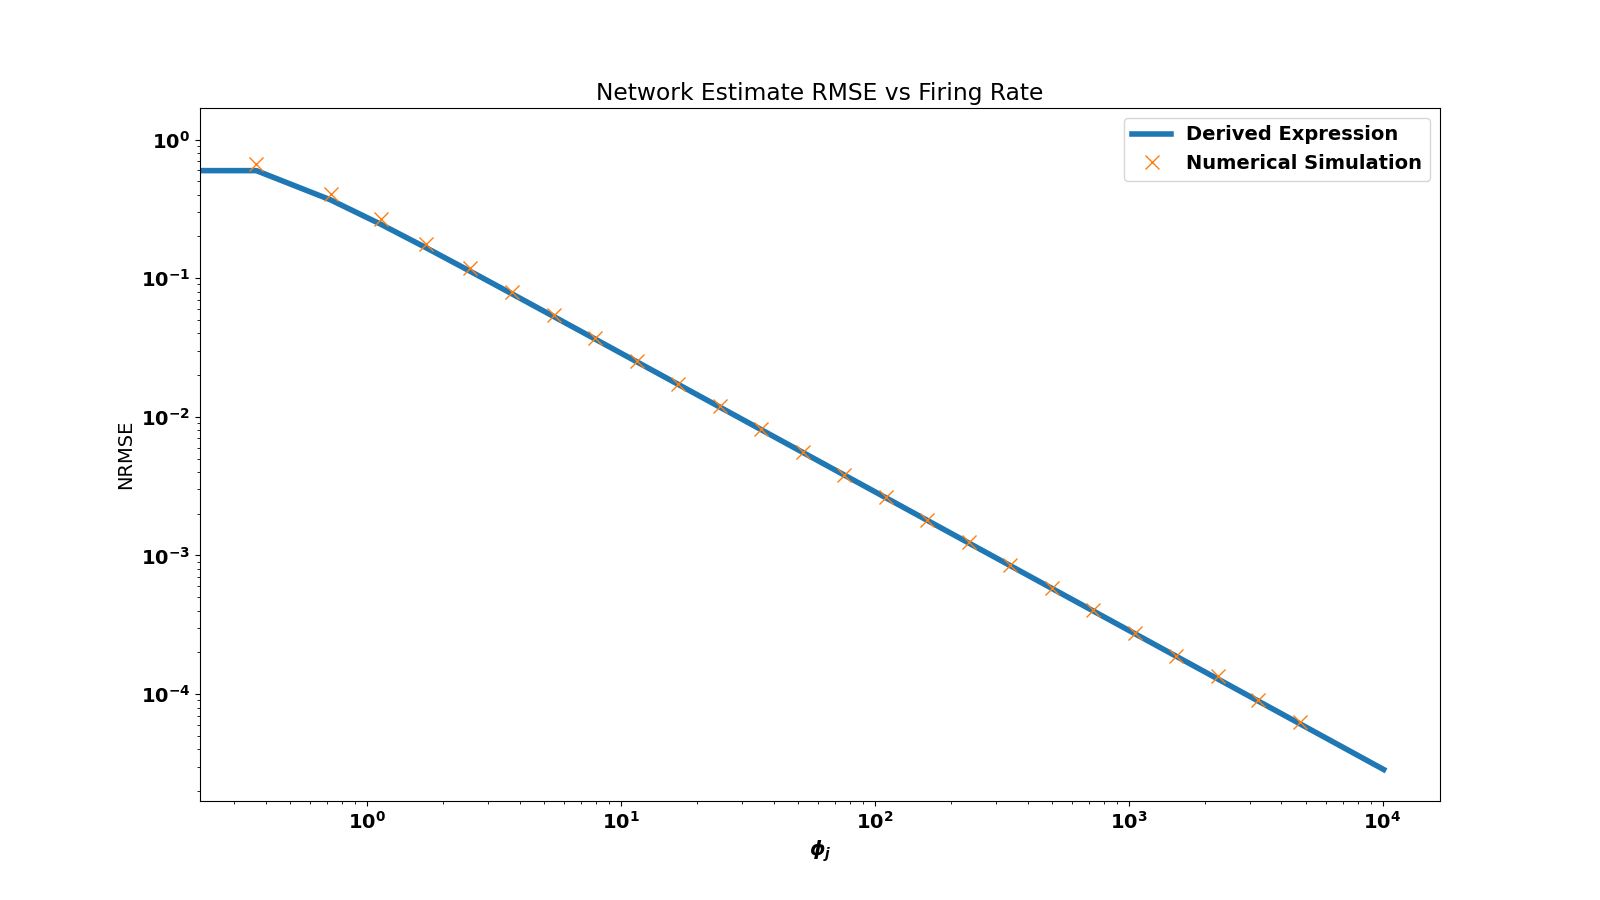
\includegraphics[width=\linewidth]{figures/per_spike_nrmse_vs_phi}
\caption{Log-log Plot of Equation (\ref{eq:const_driving:per_spike_rmse_phi}). The RMSE was computed numerically by the discrete integral $RMSE = \sqrt{\frac{1}{\phi} \sum_{i} (y - \hat{y})^2 dt}$, where $i$ sums over the data points in a spike. The integration is performed over $n = 100$ interspike intervals and averaged to form a data point. The time step was $d\xi = 10^{-4}$.}
\label{fig:const_driving:per_spike_nrmse_vs_phi}
\end{figure}

Equation (\ref{eq:const_driving:per_spike_rmse_phi}) is plotted in figure (\ref{fig:const_driving:per_spike_nrmse_vs_phi}).

\clearpage

